%poiting to the class file that has all of the information about the file
\documentclass{../lib/lib-en}
\graphicspath{ {./pc_assets/} }

% we begin the document 
\begin{document}


\customtitle{Proxy Click Email Integration}{Rene Ramirez}

\newpage
% %%%%%%%%%%%%%%%%%% %
%      STEP 1        %
% %%%%%%%%%%%%%%%%%% %
\newpage
\section*{\centering Step 1}
Open Outlook either via web or the app, 
This example uses the new version of Outlook Details will be same in any application 

\insertimage{s1.png}

% %%%%%%%%%%%%%%%%%% %
%      STEP 2        %
% %%%%%%%%%%%%%%%%%% %
\newpage
\section*{\centering Step 2}
Lets now go over to the calendar section 

\insertimage{s2.png}

% %%%%%%%%%%%%%%%%%% %
%      STEP 3        %
% %%%%%%%%%%%%%%%%%% %
\newpage
\section*{\centering Step 3}
Lets create a new event, using the \bd{"New Event"} Button

\insertimage{s3.png}

% %%%%%%%%%%%%%%%%%% %
%      STEP 4        %
% %%%%%%%%%%%%%%%%%% %
\newpage
\section*{\centering Step 4}
We now have to provide all of the following information in this tab to get the visitor meeting created

\insertimage{s4.png}

% %%%%%%%%%%%%%%%%%% %
%      STEP 5        %
% %%%%%%%%%%%%%%%%%% %
\newpage
\section*{\centering Step 5}
Provide the email addresses of all guests expected to show up, please make sure to use the correct email address as this will be used to check them in

\insertimage{s5.png}

% %%%%%%%%%%%%%%%%%% %
%      STEP 6        %
% %%%%%%%%%%%%%%%%%% %
\newpage
\section*{\centering Step 6}
Lets select this to be an In-Person event

\insertimage{s6.png}

% %%%%%%%%%%%%%%%%%% %
%      STEP 7        %
% %%%%%%%%%%%%%%%%%% %
\newpage
\section*{\centering Step 7}
Uncheck Teams Meeting as this will be an in-person event

\insertimage{s7.png}

% %%%%%%%%%%%%%%%%%% %
%      STEP 8        %
% %%%%%%%%%%%%%%%%%% %
\newpage
\section*{\centering Step 8}
Provide as much information as you want, this part is optional but will be sent as an email to the guest

\insertimage{s8.png}

% %%%%%%%%%%%%%%%%%% %
%      STEP 9        %
% %%%%%%%%%%%%%%%%%% %
\newpage
\section*{\centering Step 9}
Now we have to add proxy click into the invitation, we select the \bd{"Proxy Click"} button on the top of the menu

\insertimage{s9.png}

% %%%%%%%%%%%%%%%%%% %
%      STEP 10       %
% %%%%%%%%%%%%%%%%%% %
\newpage
\section*{\centering Step 10}
There is no log in credentials required as it is associated with your work credentials

\insertimage{s10.png}

% %%%%%%%%%%%%%%%%%% %
%      STEP 11       %
% %%%%%%%%%%%%%%%%%% %
\newpage
\section*{\centering Step 11}
Some mandatory requirements that are needed from you will now be inserted here, if your visitor requires escort in the building please make sure to select \bd{"Yes"} on the following prompt

\insertimage{s11.png}

% %%%%%%%%%%%%%%%%%% %
%      STEP 12       %
% %%%%%%%%%%%%%%%%%% %
\newpage
\section*{\centering Step 12}
This is an optional step if you need to provide any information to reception about your incoming guests

\insertimage{s12.png}

% %%%%%%%%%%%%%%%%%% %
%      STEP 13       %
% %%%%%%%%%%%%%%%%%% %
\newpage
\section*{\centering Step 13}
Lets hit \bd{"Attach"} to add proxy click into the meeting

\insertimage{s13.png}

% %%%%%%%%%%%%%%%%%% %
%      STEP 14       %
% %%%%%%%%%%%%%%%%%% %
\newpage
\section*{\centering Step 14}
Verify that the invitation to proxy click has been added with the message below and that proxy click user has been added to the recipients

\insertimage{s14.png}
\vspace{2.5cm}
\hspace{-2.2cm}
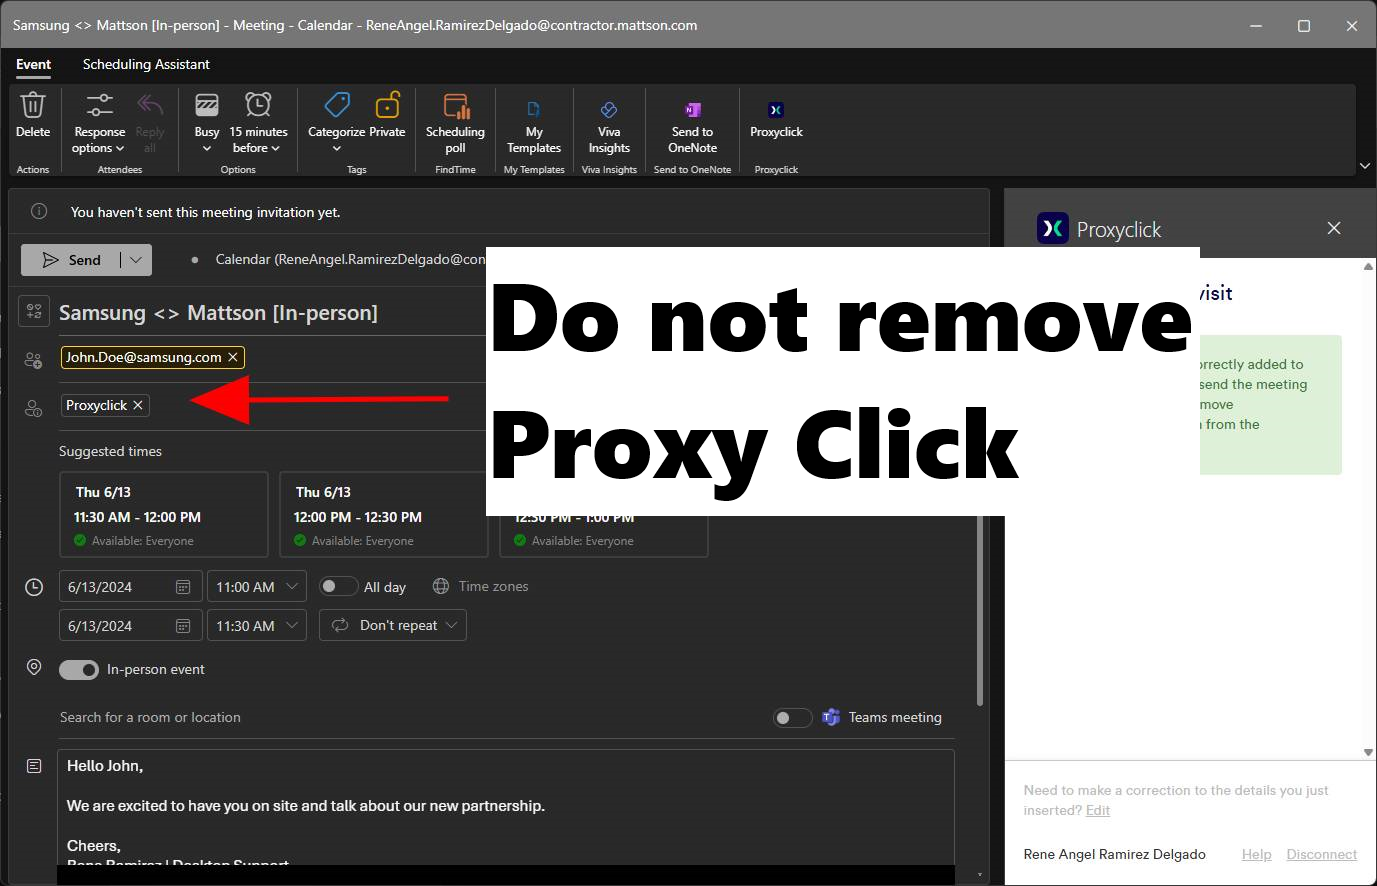
\includegraphics[width=1.3\textwidth]{s15.png}

% %%%%%%%%%%%%%%%%%% %
%      STEP 15       %
% %%%%%%%%%%%%%%%%%% %
\newpage
\section*{\centering Step 15}
Lets confirm all of the details before hitting send, but once everything is validated, simply hit \bd{"Send"}

\insertimage{s16.png}

% %%%%%%%%%%%%%%%%%% %
%      STEP 16       %
% %%%%%%%%%%%%%%%%%% %
\newpage
\section*{\centering Step 16}
Lastly verify the appointment was created by checking you calendar

\insertimage{s17.png}

\end{document}